\chapter{Method}\label{chap:method}

The method used will try to achieve the project objectives with correct results, and avoid or lower risks for project failure.


The project is a failure if the results are invalid, or cannot be realized into a real solution, or are so low quality that the project does not receive further development.
The project is also a failure if it does not provide any value for its stakeholders.


The following sections describe the key elements to the method.
There is an overarching approach, called Design Science Research.
It has 6 phases, from problem identification, to development, to evaluation and communication.
There is no methodology given by Design Science Research for executing the development phase.
Therefore, a method for this phase must be crafted from experience and existing practice.
The development phase consists of requirements engineering methods, and software development methods.


\section{Design Science Research}
%* Design Science. Build and evaluate value. Contribute to knowledge base. Is this software we need?


Design Science Research in information systems is a methodology for creating new knowledge by designing, building and evaluating software \glspl{artifact}.
It may not be as widely known as ``the scientific method'' is, and is therefore explained in more detail.

\paragraph{Design}
\textit{Design} in information systems is an iterative process and a resulting software artifact. A software artifact is to be built to solve problems for humans, and evaluated to prove it solves the problems~\cite[p.~2]{alanhevnerDesignResearchInformation2010}.


\paragraph{Research}
\textit{Research} is an activity that adds new knowledge and understanding about something.
Research should be systematical and use data to answer questions, solve problems and provide understanding~\cite[p.~2,3]{alanhevnerDesignResearchInformation2010}.

\paragraph{Design Science Research}
\textit{Design Science Research} is an approach to research where knowledge is created by design.
It is defined by \textcite[p.~5]{alanhevnerDesignResearchInformation2010} as follows:

\begin{quote}
  \textit{``Design science research is a research paradigm in which a designer answers questions relevant to human problems via the creation of innovative artifacts, thereby contributing new knowledge to the body of scientific evidence.
  The designed artifacts are both useful and fundamental in understanding that problem.''}
\end{quote}

The end goal of a Design Science Research project is to create information technology \glspl{artifact}, that improve exiting solutions or solve a problem for the first time~\cite[p.~6]{alanhevnerDesignResearchInformation2010}.
A similar methodology may also be known under the name \textit{Design and Creation}, as presented by \textcite[p.~108]{oatesResearchingInformationSystems2006}.
According to \textcite{alanhevnerDesignResearchInformation2010}, the artifacts are generally classified as \textit{constructs}, \textit{models}, \textit{methods}, \textit{instantiations} or \textit{better design theories}%
\label{par:artifact-classes}%
\footnote{This thesis aims to produce an instantiation: an implemented or prototype system. The thesis also seeks to advance on \textit{better design theories}, with regards to software architecture and protocol design.}.
A very important aspect of Design Science Research is \textit{evaluation} of the artifact.
The evaluation is the process that uncovers new knowledge, and separates the process from routine design~\cite[p.~7]{alanhevnerDesignResearchInformation2010}.
There are many aspects that could be evaluated, but the aspects that \textit{should} be evaluated are those that are related to the reason for creating the artifact in the first place; the aspects related to the research objectives~\cite[p.~115]{oatesResearchingInformationSystems2006}.


% TODO

\subsection{The General Design Cycle }

\paragraph{Design Cycle}
Problem solving by design can follow a general design cycle.
This is a circular and iterative process.
The reasoning that occurs in a design cycle, and the knowledge generated during a cycle, is illustrated in \cref{fig:dsrpm}~\cite[p.~26]{alanhevnerDesignResearchInformation2010}.

\begin{figure}[htbp]  % order of priority: h here, t top, b bottom, p page
  \centering
  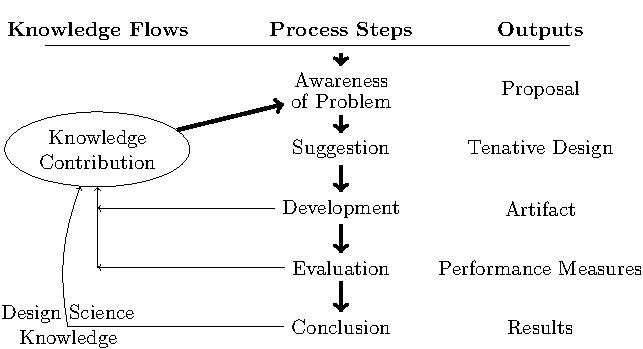
\includegraphics[width=\textwidth]{figures/dsrm-flow.pdf}
  \caption[Design Science Research Process Model]{\textbf{Design Science Research Process Model}. The general process followed by Design Science Research. Design begins with awareness of a problem, and progresses through a suggestion for a solution, to development, evaluation and a conclusion.
  The stages produce different outputs, shown in the right column.
  After the conclusion, new knowledge is contributed.
  There is also knowledge produced by development and evaluation, nicknamed ``circumscription''.
  This knowledge is fed back into a new round of suggestion~\cite[p.~11-13]{vijayvaishnaviDesignScienceResearch2019}.
  (Adopted from Figure 3 in \textcite[p.~11]{vijayvaishnaviDesignScienceResearch2019})}\label{fig:dsrpm}
\end{figure}


\paragraph{Awareness of Problem}
The process begins by becoming aware of a problem or opportunities, in the context of humans or an organization.
A proposal for what could be solved is made explicit.


\paragraph{Suggestion}
Then, a suggestion phase begins, where existing knowledge and theories are applied, as well as creativity, to create a tentative design that fits the proposal.
This design could be flawed or incorrect, which is why it is important to realize the design, to detect issues.


\paragraph{Development}
The development phase will build a solution or prototype, aiming to fulfill the suggested design.
This phase will uncover problems, inconsistencies, new learning about the problem, and other related knowledge.
That knowledge is useful for creating a new and improved design.
The quality of the \textit{implementation} of the artifact does not need to be novel, as it is the \textit{design} which is interesting~\cite[p.~12]{vijayvaishnaviDesignScienceResearch2019}.


\paragraph{Evaluation}
After an artifact is created, the evaluation phase will measure the artifact.
The measurements originate from the initial proposal, which holds the criteria for success.
This phase may also discover new knowledge, which can be used later to create a new and improved design~\cite[p.~13]{vijayvaishnaviDesignScienceResearch2019}.


\paragraph{Conclusion}
Finally, the conclusion phase will consolidate the results.
The knowledge gained from the results will either be ``firm'' or ``loose ends''.
\Textcite[p.~13]{vijayvaishnaviDesignScienceResearch2019} describes this as the following:

\begin{quote}
``\textit{Not only are the results of the effort consolidated and ``written up'' at this phase, but the knowledge gained in the effort is frequently categorized as either ``firm'' --- facts that have been learned and can be repeatedly applied or behavior that can be repeatedly invoked --- or as ``loose ends'' --- anomalous behavior that defies explanation and may well serve as the subject of further research.}''
\end{quote}


\subsection{Methodology}

Based on the understanding of design science research, and the steps of a design science research process (\cref{fig:dsrpm}), a six step Design Science Research Methodology has been made by \textcite[p.~28-30]{alanhevnerDesignResearchInformation2010}.
This methodology forms the skeleton of this thesis.
The six steps of the methodology are the following:

\begin{enumerate}
  \item \textit{Problem identification and motivation.}
  \item \textit{Define the objectives for a solution.}
  \item \textit{Design and development.}
  \item \textit{Demonstration.}
  \item \textit{Evaluation.}
  \item \textit{Communication.}
\end{enumerate}


\paragraph{1. Problem identification and motivation}
The specific research problem must be defined.
The definition is used to develop the artifact which solves the problem.
The value of a solution to the problem should be justified as well.
If the value of the solution is justified, it can motivate the researcher and the thesis' audience to pursue the solution and accept the results~\cite[p.~28,29]{alanhevnerDesignResearchInformation2010}.

\paragraph{2. Define the objectives for a solution}
The objectives should be inferred from the problem definition, and the author's knowledge of what is possible and feasible.
The objectives can be how much better a new solution should be (quantitative), or a description of how a new artifact would solve problems that are currently unsolved (qualitative)~\cite[p.~29]{alanhevnerDesignResearchInformation2010}.

\paragraph{3. Design and development}
Create an artifact to solve the problem and fulfill the objectives.
The artifact can be one of the five classes listed in \cref{par:artifact-classes} (constructs, models etc.).
The desired functionality and architecture is determined, and the actual artifact is created~\cite[p.~29]{alanhevnerDesignResearchInformation2010}.


\paragraph{4. Demonstration}
The artifact is demonstrated, to solve instances of the identified problem.
This could be experiments, simulations, case studies etc.~\cite[p.~30]{alanhevnerDesignResearchInformation2010}.


\paragraph{5. Evaluation}
The artifact is observed and evaluated to measure how well it solves the identified problem.
This can be done by comparing the results of the demonstration to the  objectives of an ideal solution.
There are many different ways to evaluate an artifact, and the correct approach should be decided based on the nature of the identified problem.
After evaluation, the researcher can go back to step 3 to improve the design.
If there is not enough time, resources or a need to do so, the process moves to step 6 instead~\cite[p.~30]{alanhevnerDesignResearchInformation2010}.

\paragraph{6. Communication}
The process must be communicated to other researchers and relevant audiences.
This communication includes: the problem and its importance, the artifact and its utility, the rigor of the artifact design, and the effectiveness of the design~\cite[p.~30]{alanhevnerDesignResearchInformation2010}.%
\footnote{This thesis is a central part of this communication.}




\section{Requirements Engineering}

In Design Science Research, there is little guidance for how to execute the actual \textit{design and development} phase.
However, the software engineering field has many approaches and ideas for how to do this.


The design of the artifact starts by gathering requirements.
These specify the concrete behaviors of the artifact; both the behaviors required for achieving the research objectives in \cref{sec:research-objectives}, and those required for a highly useable and valuable solution.


The identified requirements are both part of the design, and influence the design.
Most requirements are formed from existing knowledge of the background theory.
They are also discovered as the solution is developed.
The following subsections \ref{subsec:req-stakeholder}-\ref{subsec:req-agile} describe the key inputs for the software requirement engineering process.


\subsection{Stakeholder Discussion}\label{subsec:req-stakeholder}

Discussion with stakeholders reveal many requirements, use cases and needs.
The two key types of stakeholders here are \acrshort{EMF} experts and \gls{TDT4250} students.
The supervisor, Hallvard Trætteberg, fills the role as both a \acrshort{EMF} expert and lecturer of \gls{TDT4250}.
The author, Kristian Rekstad, fills the role as a \gls{TDT4250} student.


Dialogue questions include ``What features are required to model with \acrshort{EMF}?'' and ``What features would you like to see in a new solution?'', as well as ``Which features are missing from the existing solutions?''.


The same questions can be asked both before realizing a solution, and underway as the response to prototypes and current progress of an unfinished solution.


\subsection{Requirements Extraction}

\paragraph{Based on existing editors}
The existing tree editors in \gls{Eclipse} already implement every feature needed to do \acrlong{MDD} with the \acrlong{EMF}.
Therefore, they are excellent sources of requirements.
Especially the Sample Reflective Ecore Editor and EMF Forms Ecore Editor. %TODO: cref sections


\paragraph{No official requirements lists}
The pre-study failed to find any related research detailing requirements for a tree editor~\cite[p.~3]{rekstadModelingEnvironmentCloud2020}.
No design documents or requirements specifications were found for the \gls{Ecore} editors in \gls{Eclipse} either.


\paragraph{Use cases and requirement detection}
Therefore, the approach became to extract the requirements from the \gls{Ecore} tree editors.
The extraction is done by following use cases of modeling, as described in \cref{par:tdt4250-methodology}.
When a new functional requirement is discovered through use, it is recorded in a list.


\paragraph{Shortcomings}
This approach will find many of the required and ``obvious'' requirements.
However, hidden functionality and expert level functionality is not guaranteed to be found.
The rationale is that this functionality is not needed (yet) anyways, as the goal is to fulfil the common use cases that students have when learning \acrshort{MDD}.


There is also a risk that the user which is recording the requirements fail to detect functionality.
Some functionality can be so obvious or ``second nature'' that the user is oblivious to it.
Such functionality \textit{should} become apparent later, however, when the solution is developed and tested.
Any big omissions will prevent the use cases from succeeding.


\subsection{Source Code Analysis of Similar Projects}

\paragraph{Open source editors}
Because the tree editors for \gls{Ecore} in \gls{Eclipse} are \gls{open source}, it is possible to read and analyze the source code.
Finding the main classes responsible for editor functionality, and analyzing their method names, initialization procedures and method calls, may expose requirements.
This approach may also detect some of the more hidden functionalities, and the more ``internal'' functional requirements.


\paragraph{Architecture and software re-use}
Another advantage is that the internal architecture and patterns are exposed, which can be used to influence the artifact design.
This may increase familiarity with the design for the Eclipse ecosystem, aiding the \gls{open source} goals of this project.
It also highlights the opportunities for software re-use, when familiar code, classes, interfaces, design patterns or software libraries are used.


\paragraph{Shortcomings}
Source code analysis is dependant on analyzing the correct source code files.
If they are not found, this will fail.
This also requires the source code to have some level of quality and readability to be useful for someone not already invested in that editor code base.
The software architecture and design patterns used will matter too, in case functionality is hidden, dispersed or not clearly visible from the source code.


\subsection{Use Cases and Prototyping}

Creating realistic use cases based on \cref{par:tdt4250-methodology}, and executing them with early versions or prototypes will detect missing requirements.
This is because a user will be blocked from progressing if a critical functionality is missing.
%For example here: copy-paste, keyboard shortcuts etc)


\subsection{Agile Requirements}\label{subsec:req-agile}

\paragraph{Agile}
Core values during this thesis' requirements engineering process come from \textit{Agile}.
Agile is a counterpart to the Waterfall process\footnote{In waterfall, software is designed, developed and tested in very separate stages. All the requirements are collected, before any design or development begins. An early mistake will not be discovered until the very end of the process. Changes to requirements require a restart of the project phases.}


\paragraph{Change over Plan}
It embraces the fact that requirements change during the design and development, and thus favors \textbf{responding to change} over following a plan~\cite{kentbeckManifestoAgileSoftware2001}.
Requirements will change as they are discovered, refined and better understood later on.


\paragraph{Software over Documentation}
Another key value is that Agile prefers \textbf{working software} over comprehensive documentation~\cite{kentbeckManifestoAgileSoftware2001}.
This means that a small, working software artifact is more valuable than a large, complete and consistent list of software requirements and design, without any working software to show for it.


\paragraph{Impact of agile on requirements engineering}
The result is that the method here will start by collecting \textit{some} requirements, by using the previously described inputs.
When there are enough requirements to sufficiently solve the known use cases, design and development can begin.
There is no goal to create a complete list at the start.
The requirements are also changed, and new ones added, during the design and development.


\section{Development Methodologies}

The case for software development is the same as with requirements engineering: Design Science Research has little guidance.
And again, the software engineering field has the answers.


The goal for the development methodology is to \textbf{create the right solution}, which solves the identified problem and fulfils the software requirements.
The methodology also aims to \textbf{avoid or reduce risks} for project failure, by tackling it as early as possible.
Research often deviates from routine design here, by going for the risks first instead of delaying or hiding them, as this may lead to new knowledge~\cite[p.~114]{oatesResearchingInformationSystems2006}.


Another goal for the development process is to create ``good'', high quality software, so the project can be accepted by the \gls{open source} developer ecosystem for further development and maintenance.
Bad code or a bad design may result in a full rewrite by the next interested developer, or the developer may try to contribute but find it hard and give up.


Development methodology will not follow one strict practice, but rather piece together many different practices and values, which have lead to good results in the author's past.


\subsection{Agile}

Development will follow agile values and principles, as described in \citetitle{kentbeckManifestoAgileSoftware2001} and \citetitle{PrinciplesAgileManifesto}.
This means iterative development, rapid feedback from stakeholders, and working software.

\paragraph{Agile development}
As there are many unknown factors in development, such as third party components and services to comply and integrate with, and unknown and hard to use \glspl{API}, the plans and designs may change.
As with software requirements, the data structures, algorithms and design in the software solution will have to change as the developer learns the systems and problem space better.
\textbf{Responding to change} will be valued more than following a plan here.
Also, \textbf{working software} is more valuable than extensive documentation, meaning that code comments, tests, design specifications and diagrams will be given less effort than code, particularly if done up-front before the code.
The alternative is that this documentation is made, but the code for it quickly proves itself impossible to make, or there is not enough time to implement it, leaving only useless documentation as the result.
This also ties in to \textbf{simplicity and maximizing work-not-done}.


Regular reflection will be used weekly or bi-weekly, to assess if the process can be more effective.
Sometimes tools and technologies may seem like a good fit for the development, but instead wastes more time than the developer productivity provided.
Retrospective analysis of the development progress will try to detect this, and then expose if bad approaches are used.
If so, these will be removed or replaced if possible.


Stakeholder involvement is important as well.
The development will have a stakeholder as the developer (the author), which knows how the artifact will be used.
Additionally, the supervisor will se a demo during development, to provide feedback and help prioritize the next steps.


\subsection{Iterative Development}
* Iterative development. Work on one component at the time, up to a minimum level of functionality. Then come back later and add more.


\subsection{Lean and Minimum Viable Product}

* Lean development. Create a minimum viable product and see if it works.

\subsection{Domain Driven Design}

* Domain driven design. Increase software quality, developer understanding and software re-use with layered architecture, domain layer and ubiquitous domain language.

\subsection{Test Driven Development}

* Test driven development, where applicable. Verify behavior of critical logic, to reduce bugs and increase developer confidence and speed.

\subsection{Tracer Bullets}
* Tracer bullets. Reduce risk from integration by connecting all the major components, before developing any component fully.

\subsection{Prototyping}

* Pre-project with prototyping. Reduce risk by testing feasibility early. Creates more learning, validates requirements and discovers new requirements.


\section{Evaluation}


This section will describe how the evaluations for the artifacts were made.
The evaluations try to test for value in the solution design, by comparing how well the artifacts solve the identified problem.

\subsection{Software Artifact}

The built artifact is evaluated according to the Design Science Research methodology in \cref{par:dsrm-demonstration}.

\paragraph{Assumptions}
The functionality of the original \gls{Eclipse} editors for \gls{Ecore} is assumed to be correct and useful for students.
The functionality is also required, in order to effectively use \acrshort{EMF} for \acrfull{MDD}.

\paragraph{Demonstration goal}
Therefore, a demonstration should show the presence of the original functionality from \gls{Eclipse} in the new artifact.
To do this, the artifact will be used to complete \textit{use cases}, based on the modeling approach used in \gls{TDT4250} (see \cref{par:tdt4250-methodology}).\\


Additionally, a goal is to not use the \gls{Eclipse}, and a goal is to perform the use cases in a \gls{cloud} based \gls{IDE}, in this instance \gls{Gitpod}.


\paragraph{Evaluation of demonstration}
The evaluation%
\footnote{The evaluation is classified as \textit{ex ante} and \textit{artificial}, for those familiar with the approach by \textcite{sonnenbergEvaluationsScienceArtificial2012} and \cite{venableComprehensiveFrameworkEvaluation2012}.} 
will be a list of tests with modeling actions from \cref{par:tdt4250-methodology}.
A test is successful if the tester (the author) can perform the action, and without using \gls{Eclipse} and also doing it in \gls{Gitpod}.


\subsection{Open Source Viability}

\paragraph{Evaluation goal}
A goal of this thesis is that the artifact's source code is developed further, by either master students, the Eclipse ecosystem, or other contributors with interest in \acrshort{EMF} or tree editors.
The strategy to solve this is by making the source code \gls{open source}.


Therefore, the source code will be evaluated to indicate how fit it is to be an \gls{open source} project.


\paragraph{Test criteria}
To test how fit the project is, a checklist is synthesized from online guides for open source projects.
The sources are highly reputable, such as the Eclipse Foundation, the GitHub community, and sites endorsed by these.
The criteria will check for presence of elements or properties of the project, and succeed if it is present.
A qualitative evaluation will proceed, to conclude the test results.

